Концепция пользовательских сценариев использования является ключевым элементом в разработке программного обеспечения и системного анализа. 
Они помогают описать взаимодействие между пользователем и системой, выявить требования и ожидания к функциональности системы. 
Пользовательские сценарии не только улучшают понимание разрабатываемой системы, но и способствуют выявлению возможных проблем на ранних этапах проектирования, что позволяет сократить затраты на доработку и повысить качество конечного продукта.

Далее будут представлены конкретные сценарии, охватывающие основные функции системы.
\subsection{Пользовательские сценарии}
Прежде чем определять конкретные пользовательские сценарии, покажем высокоуровневую архитектуру системы. Она представлена на рисунке~\ref{sys_architecture}.

\begin{figure}
    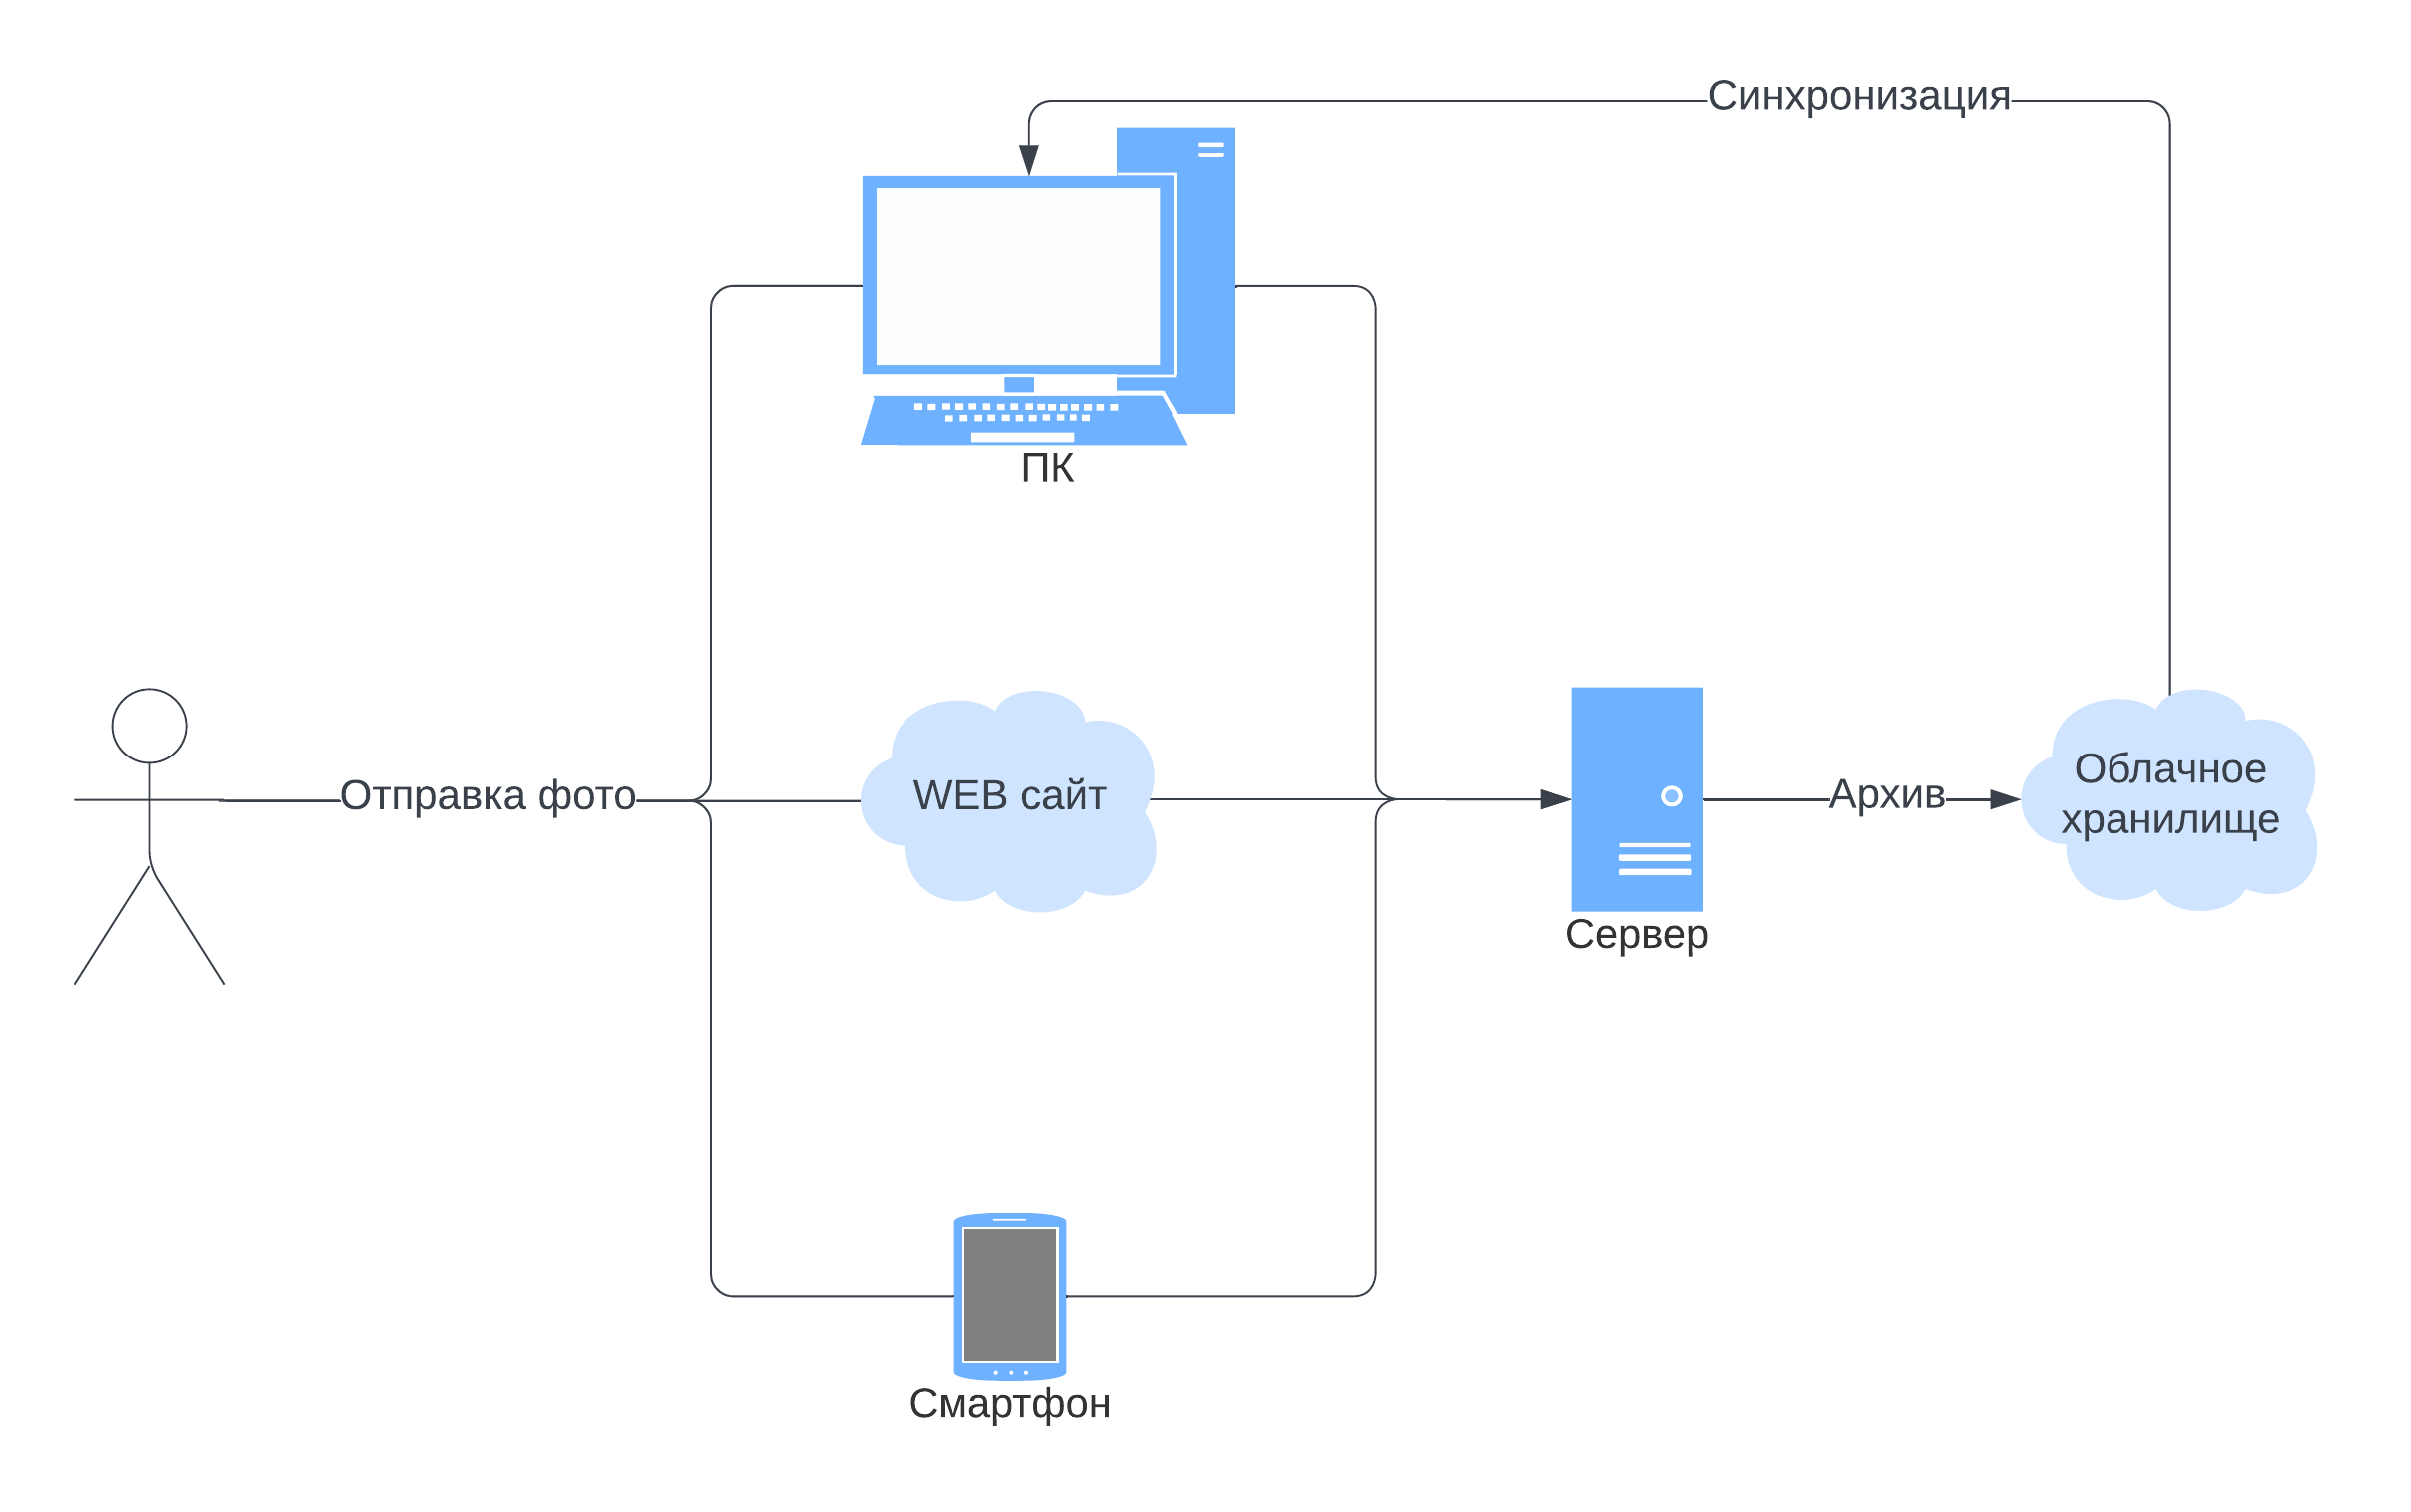
\includegraphics[scale=0.5]{img/use_cases/architecture.png}
    \caption{Высокоуровневая архитектура системы}
    \label{sys_architecture}
\end{figure}

Под пользователем приложения будем подразумевать пользователь одного из типов приложения:
\begin{itemize}
    \item веб-приложение;
    \item настольное приложение;
    \item мобильное приложение.
\end{itemize}

Для начала определим основные роли целевых пользователей:
\begin{itemize}
    \item пользователь приложения;
    \item разработчик~--- программист, занимающийся разработкой конкретных частей приложения;
    \item архитектор~--- работник, занимающийся планированием и разработкой высокоуровневой архитектуры приложения;
    \item администратор системы~--- специалист, отвечающий за настройку, управление и контроль работы системы;
    \item инженер по машинному обучению~--- специалист, занимающийся разработкой моделей машинного обучения;
    \item аналитик данных~--- специалист, занимающийся оценкой качества обучения модели, выбором подходящих метрик, а также оптимизацией процесса обучения.
\end{itemize}

\subsubsection{Авторизация пользователя}
Участники: пользователь любого из типов приложения

Предусловие: пользователь не авторизован

Постусловие: пользователь авторизован в один из сервисов и предоставлен доступ к облачному хранилищу

Сценарий:
Для авторизации в облачное хранилище необходимо реализовать следующий сценарий, изображенный на рисунке~\ref{auth}:

\begin{figure}
    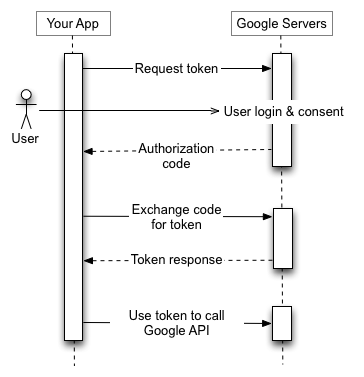
\includegraphics[scale=0.5]{img/use_cases/authorization.png}
    \caption{Сценарий сетевого взаимодействия при авторизации пользователя \cite{OAuth_google} на примере $Google$}
    \label{auth}
\end{figure}

Многие облачные хранилища предоставляют высокоуровневое $API$ для работы с ними. Также данное $API$ автоматически определяет наличие токена для авторизации, перенаправляет клиента на сайт авторизации и локально сохраняет сгенерированный токен.

\subsubsection{Преобразование фотографии}
Участники: пользователь приложения

Предусловие: пользователь сделал фото научного текста и открыл его в приложении

Постусловие: пользователь получает готовый \LaTeX--код текста и скомпилированный $pdf$ файл

Сценарий:
\begin{itemize}
    \item производится автоматическая коррекция перспективы фотографии;
    \item производится автоматическое сегментация текста на абзацы;
    \item с приложения на сервер отправляется изображение с коррекцией перспективы;
    \item с сервера на приложение отправляются координаты найденных формул;
    \item пользователь проверяет правильность распознавания формул и вносит коррективы;
    \item приложение отправляет на сервер скорректированные координаты абзацев и формул;
    \item сервер загружает \LaTeX--код и $pdf$ файлом в облачное хранилище, а также отсылает его пользователю;
    \item настольное приложение обновляет папку в облачном хранилище и загружает в локальное хранилище последний архив.
\end{itemize}

Для повышения точности пользователю предоставлена возможность корректировать точки перспективы и координаты абзацев.
\subsubsection{Преобразование файла формата \textit{.pdf}}
Участники: пользователь приложения

Предусловие: пользователь загрузил файл научного текста в формате $.pdf$ в приложение

Постусловие: пользователь получает готовый \LaTeX--код текста и скомпилированный $pdf$ файл

В случае с $.pdf$ файлом мы предполагаем, что файл является программно сгенерированным, поэтому нет необходимости корректировать перспективу.

Сценарий:
\begin{itemize}
    \item производится автоматическое сегментация текста на абзацы;
    \item с приложения на сервер отправляется изображение, а также таблица с координатами начала и конца абзацев;
    \item с сервера на приложение отправляется таблица с найденными формулами;
    \item пользователь проверяет правильность распознавания формул и вносит коррективы;
    \item приложение отправляет на сервер таблицу с финальными формулами;
    \item сервер загружает \LaTeX--код и скомпилированный $pdf$ файл в облачное хранилище, а также отсылает их пользователю;
    \item настольное приложение обновляет папку в облачном хранилище и загружает в локальное хранилище последний архив.
\end{itemize}

\subsubsection{Синхронизация между устройствами}
Участники: пользователь приложения

Предусловие: пользователь загружает фото/$pdf$ файл с мобильного устройства, пользователь авторизован в настольной версии приложения

Постусловие: пользователь получает готовый \LaTeX--код текста на настольное устройство

Сценарий:
\begin{itemize}
    \item с мобильного приложения на сервер отправляется изображение;
    \item сервер обрабатывает изображение;
    \item сервер высылает команду на синхронизацию локального хранилища настольного приложения с облачным хранилищем пользователя.
\end{itemize}

\subsubsection{Контроль обучения классификатора}

Так как самая важная часть системы (распознавание текста) реализуется на основе нейросетевых алгоритмов (о чем будет подробно рассказано позже), важно контролировать процесс обучения.
Для этого необходимо иметь доступ к метрикам модели, а также обновлять обучающие наборы данных, проводить тестирование модели на новых данных, проводить валидацию в процессе обучения.

Важно быть уверенным в том, что модель не переобучена и способна обобщать данные.

Для этих целей очень хорошо подходит платформа $\textit{Weights \& Biases}$ \cite{wandb}

Участники: аналитик данных

Предусловие: существует рабочая система, обученная модель

Постусловие: выводится информация об обучении модели

Сценарий:
\begin{itemize}
    \item пользователь заходит на веб-сайт $wandb$ \cite{wandb};
    \item пользователь выбирает интересующую его версию модели; 
    \item платформа выводит всю информацию о модели.
\end{itemize}

\subsubsection{Проверка работоспособности модели}

Участники: инженер по машинному обучению, аналитик данных

Предусловие: существует нейросетевая модель, требующая проверки

Постусловие: Модель обучена, получены необходимые метрики

Сценарий:
\begin{itemize}
    \item инженер по машинному обучению обучает модель на имеющемся наборе данных с логгированием в системе $wandb$;
    \item аналитик данных проверяет полученные метрики на удовлетворение требованиям.
\end{itemize}

\subsubsection{Замена нейросетевых моделей}

Необходимо предусмотреть возможность замены одной модели на другую. Это является важным требованием к системе, поскольку позволяет улучшать эффективность и точность работы всей системы за счет следующих преимуществ:
\begin{itemize}
    \item Возможность адаптировать систему под изменяющиеся условия: если модель устаревает или не удовлетворяет требованиям, необходимо иметь возможность быстро ее заменить.
    \item Снижение затрат на разработку и поддержку системы: вместо разработки или поддержки своей модели, можно заменить текущую модель на готовое открытое решение.
    \item Повышение гибкости системы: при изменении требований к системе, текущая модель может не удовлетворять новым требованиям.
\end{itemize}

Участники: инженер по машинному обучению, разработчик системы, аналитик данных

Предусловие: требуется замена модели

Постусловие: существует рабочая система, удовлетворяющая текущим требованиям

Сценарий:
\begin{itemize}
    \item инженер по машинному обучению разрабатывает новую модель или находит открытое решение;
    \item разработчик системы встраивает новую модель в систему;
    \item аналитик проверяет работоспособность модели;
    \item по результатам проверки:
        \begin{enumerate}
            \item в случае удовлетворения требованиям старая модель заменяется на новую;
            \item в случае неудовлетворения требованиям цикл повторяется.
        \end{enumerate}
\end{itemize}